\documentclass[10pt,a4paper]{article}
\usepackage[margin=16mm]{geometry}
\usepackage[T1]{fontenc}
\usepackage[utf8]{inputenc}
\usepackage{lmodern,amsmath,amssymb,booktabs,longtable,graphicx,xcolor,hyperref}
\hypersetup{colorlinks=true,urlcolor=blue,linkcolor=blue}
\setlength{\parskip}{5pt}\setlength{\parindent}{0pt}
\begin{document}
\begin{center}
{\LARGE\bfseries A064 v0.2.2 --- L6n1 and Triple Gear}\par
{\Large Three-core Euler flow: topology, enstrophy candidates and transport}\par
SST-Workbench numerical research prototype --- 15 October 2026
\end{center}
\begin{abstract}
Three embeddings of the same three-component Hopf-link isotopy class are studied independently:
source-native KnotPlot \texttt{link\_6.3.3} (L6n1), source-native KnotPlot \texttt{torus\_3.3} ($T(3,3)$), and
an analytic geometric centreline proxy for the Schleimer--Segerman triple gear.
The study tests whether candidate Eulerian enstrophy boundaries and tracer transport depend on embedding rather
than solely on pairwise linking. No mechanical teeth, force transmission or phase locking are simulated.
This is not a certified PKLSA dynamical provider, SST evidence, or a genuine invariant-manifold discovery.
\end{abstract}
\section{Native source and mathematical identity}
The user's Knotilus Gauss code for L6n1 is
$\{1,6,-5,-3\},\{-4,-1,2,5\},\{-6,4,3,-2\}$, i.e. Rolfsen's $6_3^3$ link.
All three components are individually unknotted, whereas each pair has $|\mathrm{Lk}_{ij}|=1$.
Both native KnotPlot sources are included with SHA-256 metadata.
Their three components are recovered from closed source-polygons separated by exceptional inter-component export jumps; per-component order is retained except for a recorded orientation reversal in L6n1 to standardize signed linking.
The Triple Gear proxy uses three congruent 120-degree rotated circles from the published geometrical arrangement
$r=0.4950197$, $\theta=-0.8560281$ rad, reflected to match the source chirality.
A common similarity scaling maps each whole link into $[-2.35,2.35]^3$, then all computational velocity fields are normalized to a common RMS speed. Those are modeling choices, not physical SST unit calibrations.
\begin{figure}[h]\centering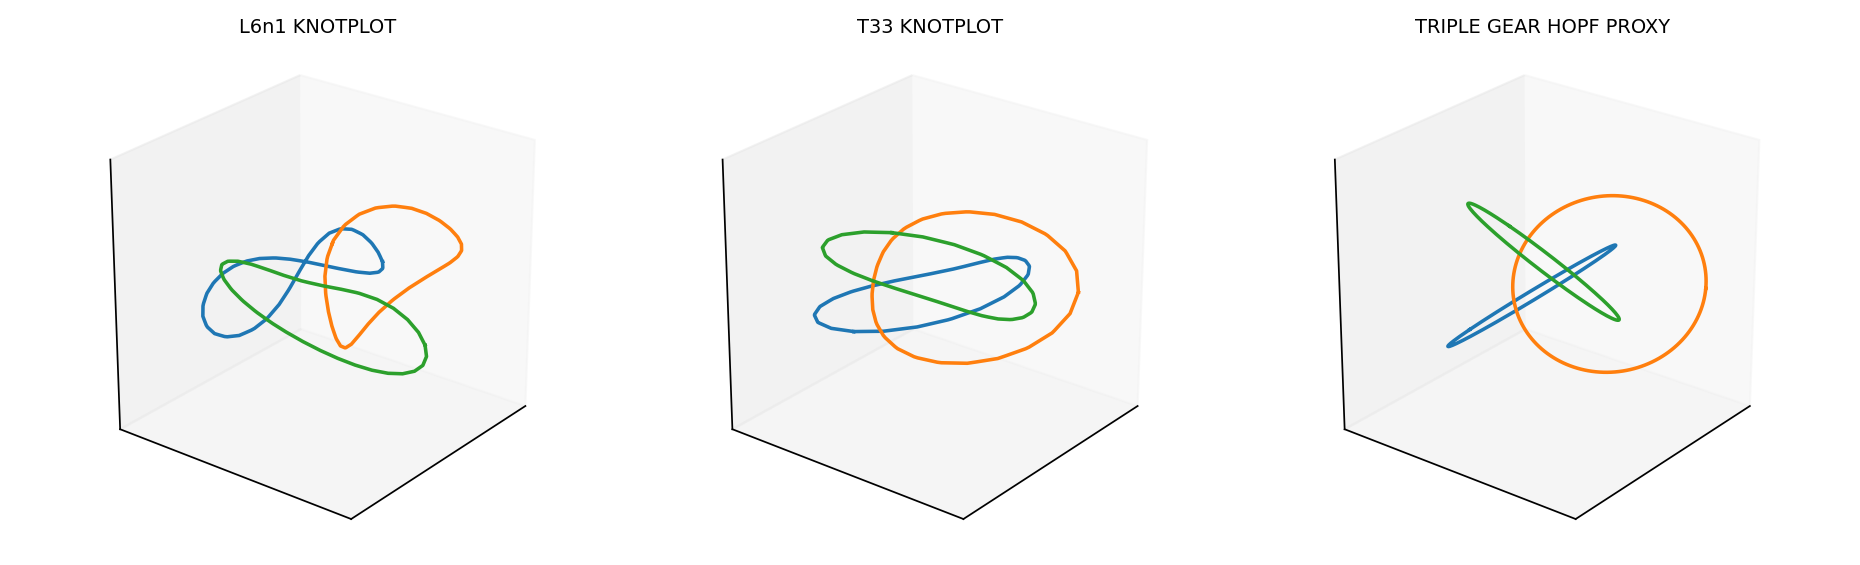
\includegraphics[width=0.98\linewidth]{THREE_HOPF_GEOMETRIES.png}
\caption{Three independently prepared Hopf-link embeddings; plot shows centerlines only.\label{fig:links}}\end{figure}
The topological qualification screens calculate three Alexander determinants equal to 1 and three Gauss-linking
integrals with magnitude approximately 1. This verifies necessary topology metrics, not a full certified link isotopy.
\section{Euler initial-value lane}
A Gaussian vorticity tube of width $a=0.42$ in a periodic $[0,2\pi]^3$ domain is laid along each source curve.
The common initial velocity is the solenoidal Biot--Savart reconstruction.
Evolution follows
\begin{equation}
\nabla\!\cdot\mathbf u=0,\qquad
\partial_t\mathbf u=\mathbb P(\mathbf u\times\boldsymbol\omega),\qquad
\boldsymbol\omega=\nabla\times\mathbf u,
\end{equation}
with Fourier pseudo-spectral RK4, $2/3$ de-aliasing, 13 saved frames over dimensionless $\Delta t=0.32$ and a bounded CFL.
Energy drift and spectral divergence are solver diagnostics, not sufficient evidence of converged tracer transport.
The native polyline geometry and initial-core conversion have no E011 anchor certificate.
\section{Discovery must precede transport}
At the first saved time step the preregistered percentiles $65,75,85,92,96,98,99,99.5$
are used to find closed, watertight isosurfaces of $|\boldsymbol\omega|^2$.
The entire discovery ledger is SHA-256 sealed before particle advection; the selected genus-one candidate is a topology-screened enstrophy feature, not an established core tube.
The independent transport stage measures
\begin{equation}
v_{n,\mathrm{rel}}=\frac{\partial_tF+\mathbf u\cdot\nabla F}{|\nabla F|},\qquad
 F(\mathbf x,t)=|\boldsymbol\omega|^2-\lambda,
\end{equation}
plus initial/final membership of RK4 advected tracers and a nearest-to-advected-core neighborhood probe.
A changing label is neither a vortex reconnection nor proof of crossing a material separatrix.
\section{Numerical outcomes}
\begin{center}\footnotesize
\begin{tabular}{lrrrrrrr}\toprule
Case & $N$ & $|\Delta E/E|$ & $Q_{95}/U$ & outer crossings & genus-1 & neighborhood & fraction\\\midrule
L6n1\_KNOTPLOT & 24 & 5.07e-11 & 0.305 & 28/224 & none & 0/192 & 0.125 \\
L6n1\_KNOTPLOT & 32 & 9.16e-12 & 0.213 & 25/221 & none & 0/192 & 0.113 \\
L6n1\_KNOTPLOT & 48 & 4.99e-12 & 0.169 & 38/224 & 99th & 0/192 & 0.170 \\
T33\_KNOTPLOT & 24 & 5.70e-11 & 0.116 & 7/224 & 85th & 0/192 & 0.031 \\
T33\_KNOTPLOT & 32 & 1.08e-11 & 0.096 & 7/224 & 85th & 0/192 & 0.031 \\
T33\_KNOTPLOT & 48 & 2.94e-12 & 0.098 & 30/224 & 85th & 0/192 & 0.134 \\
TRIPLE\_GEAR\_HOPF\_PROXY & 24 & 1.63e-11 & 0.184 & 12/221 & 98th & 0/192 & 0.054 \\
TRIPLE\_GEAR\_HOPF\_PROXY & 32 & 9.47e-12 & 0.156 & 19/224 & 98th & 0/192 & 0.085 \\
TRIPLE\_GEAR\_HOPF\_PROXY & 48 & \multicolumn{6}{c}{\textsf{NOT\_COMPLETED}} \\
\bottomrule
\end{tabular}\end{center}
\textbf{Interpretation:} The quantities above differ between distinct geometric embeddings despite common
$|\mathrm{Lk}_{ij}|=1$. A surface is not accepted as a dynamical separatrix unless
its identity persists through a resolution ladder, it remains material under particle advection, and an independent
invariant manifold or comparable transport barrier is identified.
If a genus-one candidate switches proximity-owner across grids, or first appears at a finer grid, it is
\textbf{not resolution-qualified}. A zero core-neighborhood reassignment count is only a short-time kinematic
proximity observation; it is not proof of no leakage and not an actual gear-locking observation.
\section{Falsification and unresolved gates}
\begin{enumerate}
\item Separate-source-file embedding contrast: \textbf{SCREENED}, not cross-provider qualified. Both native XYZ exports share the KnotPlot provider group.
\item Spatial/temporal/core-width convergence of tracer crossings, flux and feature surfaces: \textbf{UNRESOLVED}.
\item True material vortex tube and independently computed hyperbolic/elliptic manifold: \textbf{UNRESOLVED}.
\item Mechanical tooth-contact forces, central helix, and rational phase-lock $\theta_i=\sigma_i\kappa_i\phi+\delta_i$: \textbf{NOT MODELED}.
\item E011 STATIC\_READY matching, physical units, and framework v1.0.7 formal FREEZE/CERTIFY: \textbf{NOT EXECUTED}.
\end{enumerate}
\section{Reproduction and provenance}
\verb|run_all.cmd SELFTEST| and \verb|run_all.cmd RUN --grid 24| execute the primary lane.
\begin{verbatim}
run_all.cmd BUILD --case L6n1_KNOTPLOT --grid 32
run_all.cmd BUILD --case T33_KNOTPLOT --grid 48
run_all.cmd REPORT
\end{verbatim}
\noindent A run with \texttt{--grid 48} for the Triple Gear proxy is currently marked \texttt{NOT\_COMPLETED}.
The ZIP contains source geometry, source provenance and NPZ with source-sidecar hashes; incomplete runs are explicitly marked
\texttt{NOT\_COMPLETED}. Controls from A064 v0.2.1 (Borromean L6a4) can be compared separately, but are not claimed as the same link class.
\begin{thebibliography}{9}\small
\bibitem{KnotAtlas} Knot Atlas, ``L6n1'', \url{https://katlas.org/wiki/L6n1}.
\bibitem{Gear} S.~Schleimer and H.~Segerman (2013), ``Triple gear'', arXiv:1304.6859, \url{https://arxiv.org/abs/1304.6859}.
\bibitem{Saffman} P.~G.~Saffman (1992), \emph{Vortex Dynamics}, Cambridge University Press, DOI:10.1017/CBO9780511624063.
\bibitem{Haller} G.~Haller (2015), ``Lagrangian Coherent Structures'', \emph{Annual Review of Fluid Mechanics} 47, 137--162, DOI:10.1146/annurev-fluid-010313-141322.
\bibitem{Milnor} D.~DeTurck et al. (2013), ``Triple linking numbers, ambiguous Hopf invariants and integral formulas for three-component links'', \emph{Commun. Math. Phys.} 317, 347--370, arXiv:0901.1612.
\end{thebibliography}\end{document}
